\documentclass[times, utf8, zavrsni, numeric]{fer}
\usepackage{booktabs}
\usepackage{verbatimbox}
\usepackage{fancyvrb}
\usepackage{listings}
\usepackage{amsmath}
\usepackage[table,xcdraw]{xcolor}

\begin{document}


\thesisnumber{6487}


\title{Primjena evolucijskih algoritama u bioinformatici}


\author{Patrik Okanović
\\Voditelj: prof. dr. sc. Marin Golub}


\maketitle

% Ispis stranice s napomenom o umetanju izvornika rada. Uklonite naredbu \izvornik ako želite izbaciti tu stranicu.
\izvornik

% Dodavanje zahvale ili prazne stranice. Ako ne želite dodati zahvalu, naredbu ostavite radi prazne stranice.
\zahvala{}

\tableofcontents

\chapter{Uvod} \label{uvod}
Razvojem područja računarstva te unaprijeđenjem procesora, započinju se rješavati sve složeniji problemi koji su dotada bili nerješivi. Koriste se algoritmi  pretraživanja cjelokupnog prostora rješenja, to jest tehnika grube sile. Međutim takvi algoritmi pokazali su se poprilično nedjelotvornim i pronalazak globalnog optimuma pokazao se nerješiv u realnom vremenu. Srećom, pokazano je da nema potrebe ispitivati svaku permutaciju rješenja, što je rezultiralo pronalaskom djelotvornih algoritama. Takvi algoritmi koji pronalaze rješenja koja su zadovoljavajuće dobra, ali ne nude garanciju optimalnosti rješenja, te su im složenosti relativno niske nazivaju se heuristike. Jedna od specijalizacija heurističkih algoritama, točnije metaheuristika čiji je zadatak usmjeravanje problemski specifičnih heuristika prema području u prostoru rješenja u kojem se nalaze dobra rješenja \cite{cupicMetaheuristike},  jest područje evolucijskog računanja. Što je to evolucijsko računarstvo? Jedan od odgovora bi bio : „evolucijsko računanje je područje računarske znanosti koje razmatra algoritme koji simuliraju evolucijski razvoj vrsta, život i ponašanje jedinke u društvu ili pak simuliraju različite aspekte umjetnog života.“ \cite{neizrazito}. Bioinformatika kao izazovno područje obiluje problemima velikih složenosti. Primjena evolucijskog računarstva, posebice genetskog algoritma na neke od tih problema izložena je u nastavku.\newline

Ovaj završni rad sastoji se od 7 poglavlja. Nakon uvodnog poglavlja u \ref{genetski}. poglavlju objašnjen je genetski algoritam.\newline\newline
U \ref{bioinformatika}. poglavlju dan je pregled triju optimizacijskih problema iz područja bioinformatike te je razmotrena implementacija rješenja genetskim algoritmom.\newline\newline
Poglavlje \ref{ecf}. opisuje se razvojno okruženje za evolucijsko računanje korišteno u implementaciji rješenja.\newline\newline
Poglavlje \ref{implementacija}. izlaže rješenje optimizacijskog problema iz bioinformatike unutar odabranog razvojnog okruženja za evolucijsko računanje.\newline\newline
Unutar \ref{rezultati}. poglavlja demonstrirani su rezultati programske implementacije te je dana usporedba s rezultatima iz literature.\newline\newline
Konačno, \ref{zakljucak}. poglavlje iznosi zaključak završnog rada.




\chapter{Genetski algoritam} \label{genetski}

Evolucijsko računanje može se podijeliti u tri grane, kao što je prikazano na slici ~\ref{fig:podjelaEvolucijskog}: evolucijske algoritme, algoritme rojeva te ostale algoritme. Genetski algoritam pripada prvoj navedenoj grani evolucijskih algoritama.
\begin{figure}[htb]
	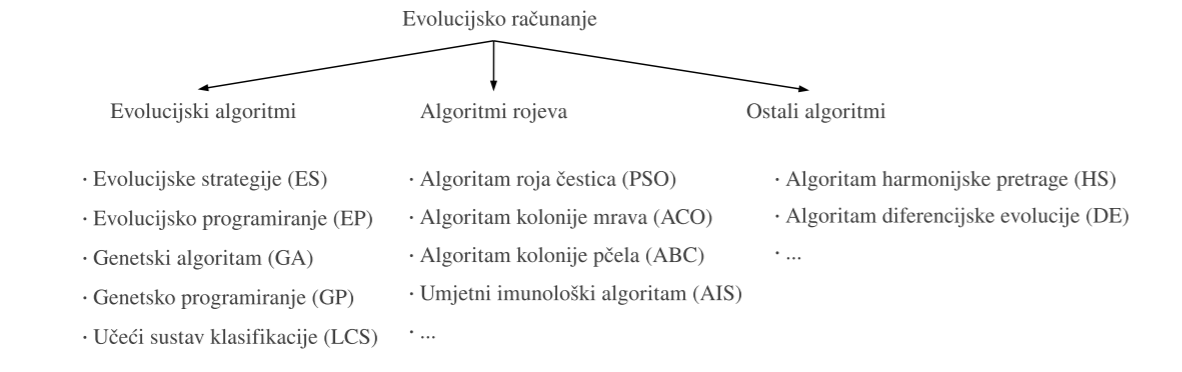
\includegraphics[width=\linewidth]{slike/podjelaEvolucijskog.PNG}
	\centering
	\caption{Hijerarhijski prikaz evolucijskog računanja}
	\label{fig:podjelaEvolucijskog}
\end{figure}

Kroz milijune godina različite vrste se razvijaju kako bi što bolje preživjele u okolišu oko njih. Razvijene prilagodbe se prenose unutar vrste generacijama, te je proces prilagodbe kontinuirani proces. Prilagodbe su većinom takve da omogućuju jedinki bolje šanse za preživljavanje, iako postoje i nepogodne promjene. Štetne promjene generacijama postepeno iščezavaju, dok promjene koje su korisne imaju veće šanse za očuvanjem unutar populacije jer povećavaju šanse jedinke za preživljavanjem. Opisani mehanizam jest način prirode za razvijanjem sve sposobnijih organizama.

"Genetski algoritam je heuristička metoda optimiranja koja imitira prirodni evolucijski proces." \cite{gaSkripta}. Genetski algoritmi predloženi su od strane Johna H. Hollanda 1970-ih godina. Primjenjuju se za rješavanje optimizacijskih problema, štoviše koristi se uz dobre rezultate pri učenju neuronskih mreža, traženju najkraćeg puta, problemu trgovačkog putnika, strategiji igara, problemima sličnim transportnom problemu, optimiranjima nad bazom podataka te u mnogim drugim problemima. Genetski algoritam modelira prirodni genetski sustav: 
\begin{itemize}
	\item genetski materijal jedinke zapisan je u strukturi zvanoj kromosom,
	\item nad populacijom se vrše genetski operatori: križanje i mutacija,
	\item događa se selekcija.
\end{itemize}
Pseudokod genetskog algoritma dan je na ~\ref{pseudoGen}.
\begin{figure}[h]
\begin{verbatim}
Genetski_algoritam
{
   t = 0
   generiraj početnu populaciju potencijalnih rješenja P(0);
   sve dok nije zadovoljen uvjet završetka evolucijskog procesa 
   {
      t = t + 1;
      selektiraj P'(t) iz P(t-1);
      križaj jedinke iz P'(t) i djecu spremi u P(t);
      mutiraj jedinke iz P(t);
   }
   ispiši rješenje;
}
\end{verbatim}
\caption{Pseudokod genetskog algoritma}
\label{pseudoGen}
\end{figure}

Za genetski algoritam jedinke su potencijalna rješenja, a okolinu predstavlja funkcija cilja. Ukoliko postoji potreba za implementiranjem genetskog algoritma kao metode optimiranja, potrebno je definirati proces dekodiranja i preslikavanja podataka zapisanih u kromosomu te odrediti funkciju dobrote.

Neke od mogućnosti prikaza rješenja genetskog algoritma su:
\begin{itemize}
	\item prikaz rješenja s pomoću binarnog koda, to jest binarni prikaz,
	\item prikaz s Grayevim kodom,
	\item kromosom kao broj s pomičnom točkom,
	\item matrični prikaz.
\end{itemize}

Funkcija dobrote u literaturi zvana \textit{fitness} funkcija ili funkcija ocjene kvalitete jedinke je ključ za proces selekcije. Što je kvaliteta jedinke veća uz pomoć funkcije dobrote ta jedinka će imati veću šansu za preživljavanje. 

Selekcijom se čuvaju i prenose dobra svojstva jedinki na sljedeću generaciju u populaciji. Genetske algoritme s obzirom na vrstu selekcije dijelimo na generacijske i eliminacijske. Karakteristične vrste selekcija koje koristi generacijski genetski algoritam su: jednostavna selekcija i turnirska selekcija.

U praktičnom dijelu ovog rada koristi se 3-turnirska eliminacijska selekcija.
3-turnirska eliminacijska selekcija odabire slučajno tri različite jedinke iz populacije i eliminira najlošiju jedinku za razliku od 3-turnirske generacijske selekcije koja kopira najbolju jedinku u novu populaciju. Vjerojatnost eliminacije \textit{t}-te jedinke uporabom 3-turnirske selekcije iznosi 
\[p_{3,E}(i) = \frac{\binom{i}{3} - \binom{i-1}{3}}{\binom{N}{3}}\] 
Tri jedinke iz skupa od N jedinki moguće je odabrati na $\binom{N}{3} $načina. Najlošija jedinka od tri odabrane ima najveću oznaku. Ukolika je odabrana \textit{i}-ta jedinka sve ostale jedinke moraju imati manji ili jendaki indeks. Vjerojatnost da su slučajno odabrane jedinke u skupu od prvih \textit{i} iznosi $\frac{\binom{i}{3}}{\binom{N}{3}}$. Konačno od te vjerojatnosti potrebno je oduzeti vjerojatnost da sve tri jedinke imaju indeks manji od \textit{i}, a to iznosi $\dfrac{\binom{i-1}{3}}{\binom{N}{3}}$.

\section{Utjecaj operatora}
Neovisno o tome koja inačica genetskog algoritma se koristi, operatori mutacije i križanja imaju značajnu ulogu.

Operator križanja na temelju roditelja stvara djecu. Zbog toga što su djeca slična roditeljima, ovaj operator ima ulogu fine pretrage prostora rješenja u okolici rješenja koja reprezentiraju roditelji.

\begin{figure}[htb]
	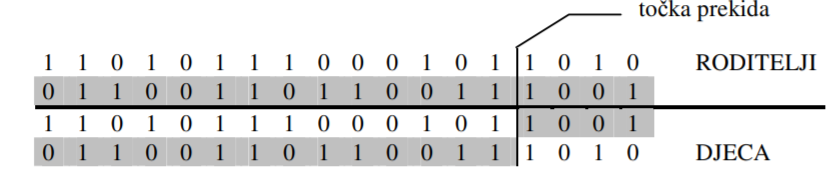
\includegraphics[width=\linewidth]{slike/crossover2.PNG}
	\centering
	\caption{Križanje s jednom točkom prekida}
	\label{fig:crossover2}
\end{figure}

Slika ~\ref{fig:crossover2} prikazuje često korišteni operator križanja s jednom točkom prekida prilikom korištenja binarne reprezentacije jedinke. Slučajno se odabire točka prekida unutar jedinki. Kromosomi roditelja prelamaju se na točki prekida i tvore djecu. Prvo dijete prvi dio kromosoma dobiva od prvog roditelja, a drugi dio od drugog roditelja. Drugo dijete prvi dio kromosoma dobiva od drugog roditelja, a drugi dio kromosoma od prvog roditelja.

Operator mutacije ima suprotnu ulogu, on nad jedinkom radi  jednu ili više slučajnih izmjena koje jedinku mogu drastično izmijeniti . Ovaj operator povećava volumen populacije u postupku pretraživanja. Druga bitna uloga operatora mutacije jest izbacivanje populacije iz lokalnih optimuma.

\begin{figure}[htb]
	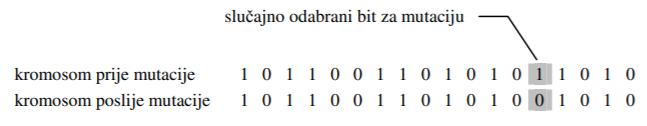
\includegraphics[width=\linewidth]{slike/mutacijaPr.PNG}
	\centering
	\caption{Jednostavna mutacija \cite{gaSkripta}}
	\label{fig:mutacija}
\end{figure} 

Slika ~\ref{fig:mutacija} prikazuje jednostavnu mutaciju prilikom korištenja binarne reprezentacije jedinke. Svaki bit kromosoma mutira s odabranom vjerojatnošću \textit{p}. Postoje brojne mutacije koje je moguće koristiti. Odabir mutacije mora odgovarati problemu koji se rješava. Neki od primjera operatora mutacije nad binarnim kromosomom mogu biti: invertiranje svih bitova ili mutiranje točno određenog broja slučajnih pozicija u kromosomu.

Kako bi genetski algoritam bio djelotvoran potrebno je postići dobar balans između operatora križanja i operatora mutacije. Ukoliko je djelovanje križanja prejako, postupak može vrlo lako zaglaviti u lokalnome optimumu. Ako je djelovanje mutacije prejako, može se dogoditi da mutacija uništava sve pozitivno što je algoritam dotada pronašao, što svodi pretragu na slučajnu. U idealnoj situaciji, ovi operatori u balansu osiguravaju da algoritam pretraživanja napreduje prema kvalitetnijim rješenjima.


\chapter{Optimizacijski problemi iz bioinformatike} \label{bioinformatika}

Prije predstavljanja tri optimizacijska problema iz bioinformatike dan je uvod u osnove genomike te korišteni format podataka u implementaciji rješenja. Predstavljeni optimizacijski problemi su:
\begin{enumerate}
	\item Populacijska genetika u kojoj je potrebno simulirati prirodni tijek razmnožavanja i evolucije te pratiti samo najvjerojatnije ishode u kojima se unutar populacije održavaju dominantna svojstva
	\item Genetsko predviđanje kojim je potrebno odrediti položaj kodirajućeg gena u slijedu.
	\item Poravnanje više sljedova odjednom kao što naziv kaže potrebno je dane DNK ili RNK sljedove nadopuniti prazninama te poravnati uz najveće moguće preklapanje.
\end{enumerate}

\section{Osnovni pojmovi u području genomike}
Genomika je grana genetike koja primjenjuje metode DNA sekvenciranja te bionformatike
kako bi ostvarila sekvenciranje, sastavljanje i analizu funkcija i strukture genoma. 

Bipolimeri su presudne makromolekule nukleinskih
kiselina, proteina i ugljikohidrata za funkcioniranje živih bića. Temeljne vrste nukleinskih kiselina su: RNA i DNA. Dok DNA služi kao spremište instrukcija za razvoj i funkcioniranje
živih organizama, RNA dijelimo na nekoliko vrsta ovisno u funkciji. Tako postoji glasnička RNA (mRNA), transportna RNA (tRNA), ribosomska (rRNA) te regulacijske RNA poput mikro RNA (miRNA), male jezgrene RNA (snRNA) i male interferirajuće RNA (siRNA).  

Osnovna jedinica nasljeđivanja živih organizama jest gen. Gen je dio nukelinske kiseline koji kodira informaciju za proizvodnju proteina ili RNA lanaca koji imaju aktivnu funkciju u organizmu.

DNA molekule su dvostruke uzvojnice koje se sastoje od nukleotida. Nukleotidi se sastoje od nukleinskih baza A (adenin), C (citozin), G (gvanin),  T (timin), potom od naizmjeničnog niza šećera i fosfatne skupine. Lanci DNA povezani su na način da se adenin spaja s timinom, a gvanin s citozinom.

\section{Format podataka FASTA}
FASTA je najčešći oblik podataka u bioinformatici. FASTA je tekstualni format koji služi za prikazivanje sljedova proteina ili nukleinskih kiselina pri čemu je svaki nukleotid ili aminokiselina prikazana jednim slovom. U tablici ~\ref{fastaTablica} dan je prikaz svih mogućih kodova unutar FASTA zapisa podataka.

\begin{table}[h]
	\centering
	\begin{tabular}{|c|c|}
		\hline
		\rowcolor[HTML]{C0C0C0} 
		\multicolumn{1}{|l|}{\cellcolor[HTML]{C0C0C0}\textbf{Kod nukleinske kiseline}} & \textbf{Značenje}               \\ \hline
		A                                                                              & Adenin                          \\ \hline
		C                                                                              & Citozin                         \\ \hline
		G                                                                              & Gvanin                          \\ \hline
		T                                                                              & Timin                           \\ \hline
		U                                                                              & Uracil                          \\ \hline
		R                                                                              & A ili G                         \\ \hline
		Y                                                                              & C, T ili U                      \\ \hline
		K                                                                              & G, T ili U                      \\ \hline
		M                                                                              & A ili C                         \\ \hline
		S                                                                              & C ili G                         \\ \hline
		W                                                                              & A, T ili U                      \\ \hline
		B                                                                              & ne A (npr. C, G, T ili U)       \\ \hline
		D                                                                              & ne C (npr. A, G, T ili U)       \\ \hline
		H                                                                              & ne G (npr. A, C, T ili U)       \\ \hline
		V                                                                              & niti T niti U (npr. A, C ili G) \\ \hline
		N                                                                              & A C G T U                       \\ \hline
		X                                                                              & Maskiranje                      \\ \hline
		-                                                                              & Praznina/procjep                \\ \hline
	\end{tabular}
\caption{Kodovi za prikaz nukleinskih kiselina u FASTA formatu}
\label{fastaTablica}
\end{table}

U FASTA datoteci može biti više zapisa, a svaki zapis sastoji se od linije zaglavlja te jedne ili više linija samog slijeda. Linije komentara poćinju znakom ",". Primjer FASTA datoteke: 

\begin{verbbox}
>Prvi slijed
AGCCTGCT-CGT
>Drugi slijed
AGCTATAGCTAGA
>Treci slijed
AGCTATCCTAAGCG
\end{verbbox}
\begin{figure}[ht]
	\centering
	\theverbbox
	\caption{Primjer FASTA datoteke}
\end{figure}

\section{Populacijska genetika}
Populacijska genetika (engl. \textit{Population Genetics}) proučava distribuciju alela. Aleli, homologni geni, elmorfi naziv su za dva alternativna gena koja određuju istu osobinu, a u stanicama  uvijek dolaze u paru. Distribucija alela uzrokovana je četirima faktorima koji definiraju evoluciju, a to su: 
\begin{enumerate}
	\item Prirodna selekcija.
	\item Genetski drift, označava promjenu u frekvenciji genetske varijacije određenog alela. Događa se uslijed nasumičnog "nestajanja" gena primjerice razmnožavanjem ili bilo kojim drugim uzrokom koji sprječava da se gen za određeno svojstvo prenese na iduću generaciju.
	\item Mutacije.
	\item Tok gena, prijenos gena iz jedne populacije u drugu.
\end{enumerate}


Za bolje razumijevanje populacijske genetike, u nastavku su iznesene biološke osnove.
Genotip je genska osnovica organizma, njena genska struktura odnosno svi geni koji ga čine. Fenotip je svaka vidljiva karakteristika jedinke. U primjeru boja latica, fenotip bi bio stvarna boja latica koju vidi promatrač. Jedan gen određuje boju latica, iako aleli koji tvore gen mogu biti različiti. 
Diploidni organizmi poput ljudi, posjeduju dvije kopije svakog kromosoma, jednu kopiju od majke, a drugu od oca. Geni imaju jedan alel od prvoga kromosoma, te drugi alel od drugog kromosoma. Aleli mogu biti recesivni ili dominantni. Za gen s dva alela, gdje je R dominatno svojstvo, a r recesivno svojstvo, moguće su tri kombinacije: Rr, RR, rr. Veza genotipa i fenotipa opisuje se tako da genotip plus utjecaj okoline daje fenotip. Genotip je moguće saznati gledajući DNK, dok je fenotip moguće utvrditi promatranjem jedinke. Lewontin 1974. predlaže sljedeći opis cilja preslikavanja "genetskog i fenotipskog prostora" \cite{applicationOfBioinformatics} :\newline
"Izazov teorije populacijske genetike je pružiti skup pravila pomoću kojih je moguće predvidjeti preslikavanje populacije genotipa G1 u domenu fenotipa P1, gdje postoji selekcija, te drugi skup pravila koje preslikavaju P1 u skup fenotipa P2, te ponovno u domenu genotipa G2." 
\begin{center}
G1 $\rightarrow$ P1 $\rightarrow$ P2 $\rightarrow$ G2
\end{center}
Složenost problema je eksponencijalna \cite{applicationOfBioinformatics}, zbog toga je prikladno primijeniti genetski algoritam.

Genetskim algoritmom moguće je simulirati populacijsku genetiku uz pseudonepredvidljive uvjete. Pitanje na koje se želi odgovoriti eksperimentom: može li promatranje prethodnih tokova gena pomoći u predviđanju budućih generacija?

Moguća implementacija rješenja od korisnika bi tražila unos broja alela koje je potrebno pratiti. Dopuštene kombinacije alela bilo bi moguće zadati konfiguracijskom datotekom uz ostale parametre koji simuliraju uvjete u prirodi, poput svojstva dominacije, recesivnosti, pojedine vjerojatnosti i mnoge druge. Za svaku populaciju bilo bi potrebno pratiti frekvencije alela. Praćenjem frekvencije alela ostvario bi se uvid u tok gena te bi bila dana sposobnost predikcije svojstava budućih naraštaja. Primjerice bez dodatnih ograničenja ukoliko bi korisnik zadao alele : \{0, 1, 2, 3\}. Postoje \(4^2\) kombinacije alela. Izradom različitih funkcija dobrote koje bi bile naklonjenije pojedinim alelima približno bi se modelirali uvjeti prirode. U radu \cite{applicationOfBioinformatics} korišten je generacijski genetski algoritam s jednostavnom selekcijom. Jedinka predstavlja par alela te je u implementaciji reprezentirana binarnim prikazom. Korišteni operator križanja je križanje s jednom točkom prekida, a korišteni operator mutacije je jednostavna mutacija kojom se mijenjaju slučajno odabrani bitovi unutar reprezentacije jedinke. Iz slika ~\ref{fig:popPrva} i ~\ref{fig:popDruga} rezultata rada \cite{applicationOfBioinformatics} moguće je zaključiti promatranjem frekvencija koji geni su dominantni (0 i 2), a koji recesivni (1 i 3). Kroz sve veći broj iteracija stvaranjem novih generacija, dominanta svojstva postaju zastupljenija, a recesivnim se frekvencija pojavljivanja smanjuje. 
\begin{figure}[!httb]
	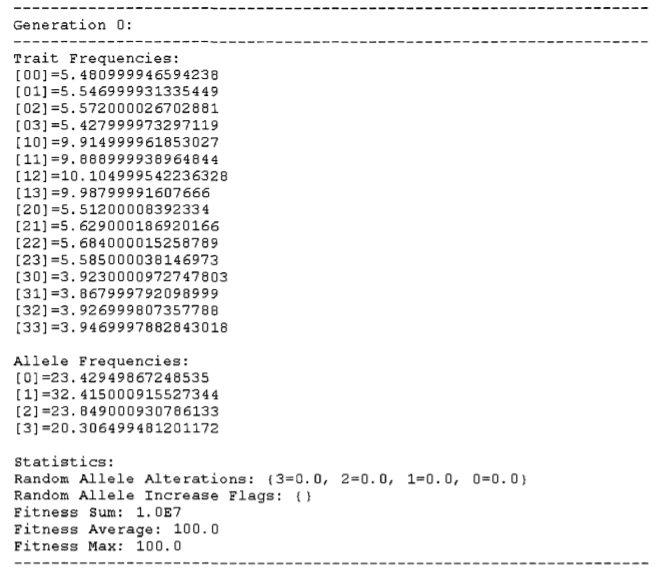
\includegraphics[]{slike/popPrva.PNG}
	\centering
	\caption{Početna populacija}
	\label{fig:popPrva}
\end{figure}

\begin{figure}[!httb]
	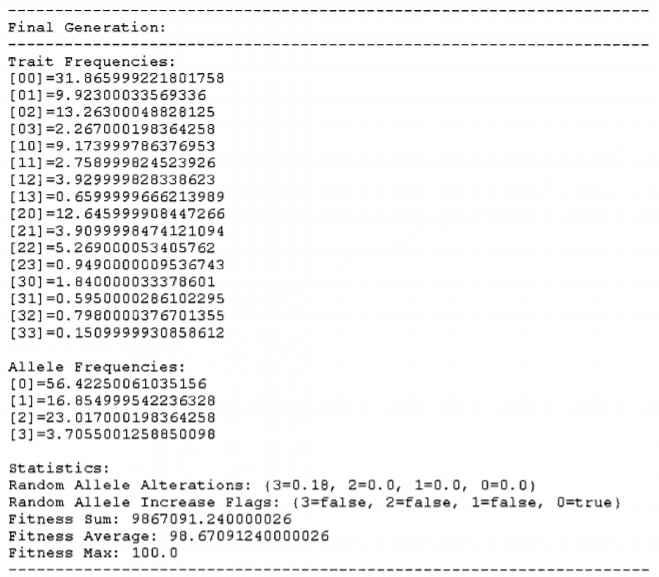
\includegraphics[]{slike/popDruga.PNG}
	\centering
	\caption{Završna populacija}
	\label{fig:popDruga}
\end{figure}
\newpage
\section{Genetsko predviđanje}
Genetsko predviđanje(engl \textit{gene prediction, gene finding}) jedan je od najizazovnijih problema bioinformatike. Cilj je genetskog predviđanja identificirati područja u lancu koja će kodirati proteine. Kodiranje slijeda dušičnih baza jedno je od temeljnih spoznaja u biologiji. Niz od tri dušične baze tvori kodon. Postoje 64 moguće kombinacije kodona, neke kombinacije predstavljaju početak proteina i takvi kodoni nazivaju se start kodoni, sukladno tome neke kombinacije označavaju kraj te ih nazivamo stop kodonima. Različite permutacije kodona počevši sa start kodonima, a završavajući sa stop kodonima tvore različite bjelančevine. Zbog toga što je iz dana u dan sekvencirano sve više genoma, potreba za djelotvornom analizom tih lanaca postaje sve veća. 

Prvi korak analize jest locirati kodirajuća i nekodirajuća područja sekvenci RNK, odnosno egzone i introne. Egzoni su uz introne dijelovi koji tvore RNK slijed, razlika između egzona i introna jest u tome što egzoni kodiraju proteine. Prema tome u stanici se mRNK prelama na dodiru introna i egzona i nakon toga samo egzoni kodiraju proteine. Metode je moguće podijeliti u dvije kategorije: pretraživanja po sličnosti te \textit{ab initio} predviđanja. Slika ~\ref{fig:strukturaGena} prikazuje strukturu gena.

\begin{figure}[htb]
	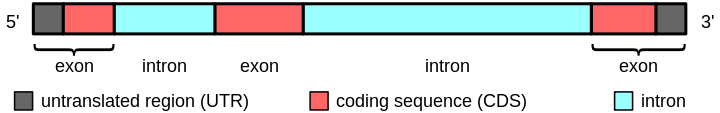
\includegraphics[width=\linewidth]{slike/genePrediction.PNG}
	\centering
	\caption{Struktura gena \cite{wikiGen}}
	\label{fig:strukturaGena}
\end{figure}

Empirijskim metodama pronalaska gena potrebno je pronaći genom sekvenci kojim se može identificirati područje uz pomoć mRNK, tvorevinama proteina, homolognim ili ortogonalnim nizovima. Uz mRNK sekvencu, trivijalno je otkriti otkuda se dogodila transkripcija \cite{applicationOfBioinformatics}. Pomoću danog proteinskog slijeda, moguće je pronaći familiju kodirajućih DNK sekvenci reverznim prevođenjem genetskog koda. Nakon sekvenciranja, algoritmi lokalnog poravnjanja poput algoritma BLASTA i algoritma Smith-Waterman pretražuju područja sličnosti između dijela DNK i potencijslnih kandidata. Uspješnost ovakvog načina ograničena je ispravnošću baze poznatih sekvenci. 

\textit{Ab initio} (lat. \textit{od početka}) genetsko predviđanje je intrinzična metoda zasnovana na detekciji signala i sadržaja. Primjeri signala su: start kodoni, stop kodoni, točke grananja. Algoritmi poput dinamičkog programiranja, linearne analize diskrimanti, Linguist metode, skrivenih Markovljevih modela te neuronske mreže koriste se u \textit{ab initio} metodi pronalaženja gena. 
 Općenito u algoritmima za predviđanje gena prvo je potrebno identificirati ORF (engl. \textit{Open Reading Format}). ORF se može objasniti kao dio slijeda kojeg je moguće prevesti. Prevođenje u biologiji odgovara postupku u kojem stanični ribosomi sintetiziraju proteine nakon transkripcije RNK u DNK. Jedan od mogućih načina kako prepoznati ORF jest sljedeći: za pretpostavljene ORFove na promatranome slijedu napraviti prevođenje danoga slijeda u aminokiselinu pomoću baze podataka ORFova te nakon toga tu aminokiselinu potražiti u drugoj bazi podataka \cite{applicationOfBioinformatics}. Postojeći programi koji služe za prepoznavanje ORFa su BioEdit, DNA STRIDER, PLOTORF, GETORF... 
\begin{figure}[htb]
	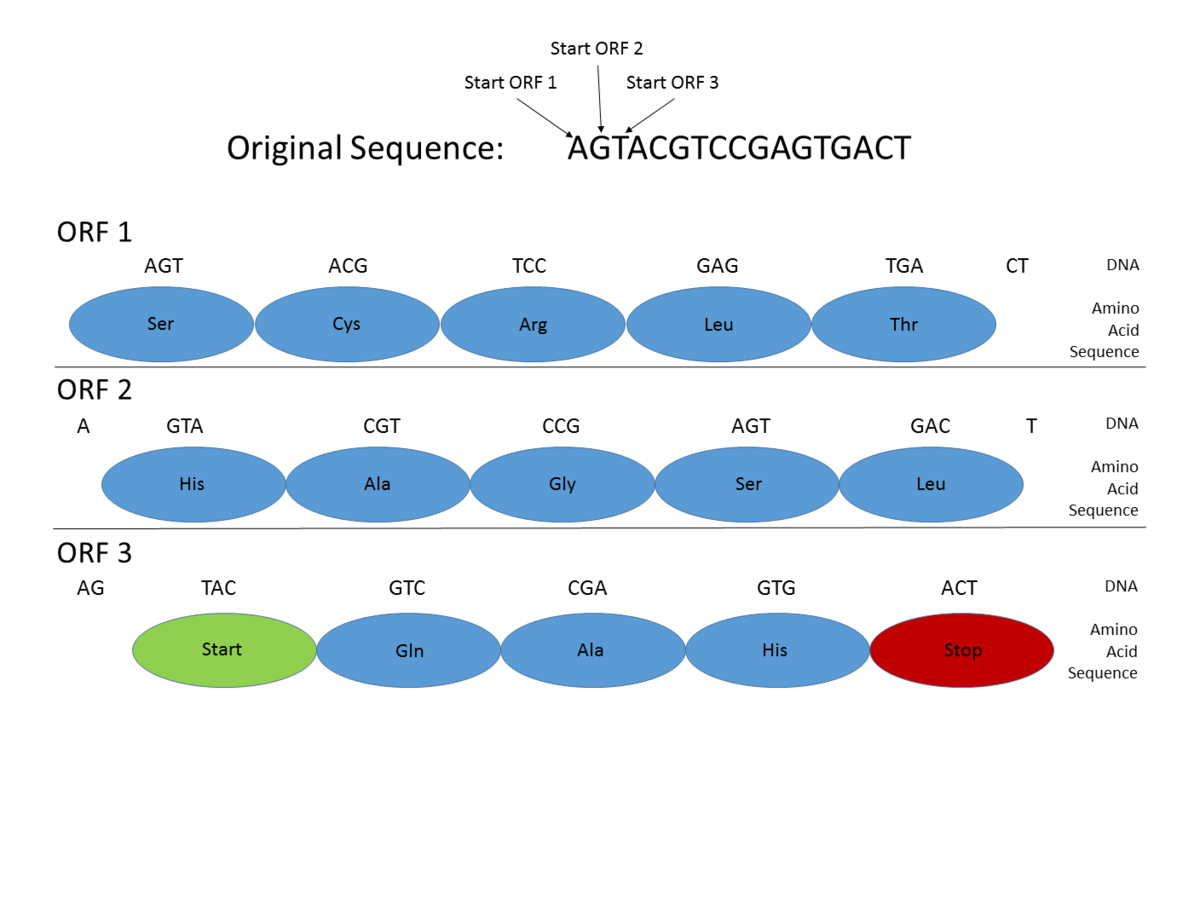
\includegraphics[width=\linewidth]{slike/ORF.PNG}
	\centering
	\caption{Prepoznavanje ORFa \cite{wikiORF}}
	\label{fig:prepoznavanjeORF}
\end{figure}
Slika ~\ref{fig:prepoznavanjeORF} prikazuje postupak predviđanja gena prepoznavanjem ORFova, određuju se moguće granice početka kodiranja slijeda. Funkcionalni proteini moraju započeti sa start kodonom (gdje započinje transkripcija DNA), a završavaju sa stop kodonom (gdje se transkripcija završava). Gledajući gdje ti kodoni mogu pasti u slijedu DNK, može se vidjeti gdje se može nalaziti funkcionalni protein. Ovo je važno u predviđanju gena, jer može otkriti gdje se kodiraju geni u čitavom genomskom slijedu. U ovom primjeru, funkcionalni protein može se otkriti pomoću ORF3, jer započinje s početnim kodonom, ima više aminokiselina, a zatim završava stop kodonom, a sve unutar istog okvira za čitanje, to jest ORFa.
Moguće rješenje uporabom genetskog algoritma nalazi se u \cite{applicationOfBioinformatics}.   
Inicijalna populacija generirana je dijeljenjem dane DNK sekvence u slučajni broj dijelova. Križanje jedinki ostvareno je križanjem s jednom točkom prekida. Prilikom križanja implementacija provjerava da se točka prekida ne nalazi usred kodirajućeg područja DNK.

\begin{figure}[htb]
	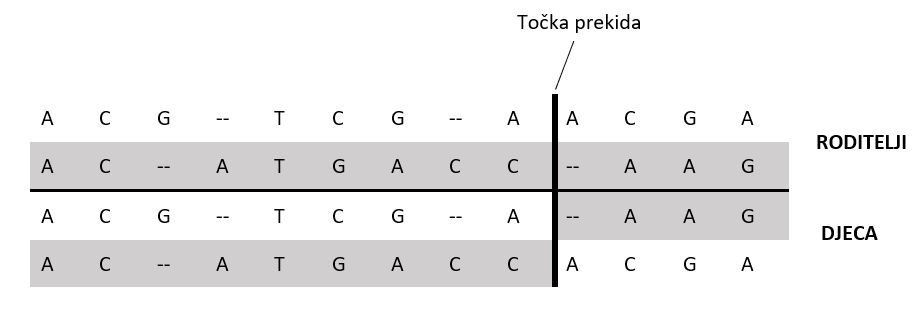
\includegraphics[width=\linewidth]{slike/crossover.PNG}
	\centering
	\caption{Križanje s jednom točkom prekida}
	\label{fig:crossover}
\end{figure}
Na slici ~\ref{fig:crossover} prikazano je križanje s jednom točkom prekida. Mutacijom jedinke pokušava se prepraviti ukoliko je DNK sekvence prekinuta usred egzona. Najbitniji dio implementacije genetskog algoritma je funkcija dobrote. Funkcija dobrote uzima u obzir frekvenciju kodona te frekvenciju područja G+C nasuprot frekvenciji područja A+T, te potom kreira nehomogene Markovljeve modele za kodirana područja \cite{applicationOfBioinformatics}. Algoritam izračunava vjerojatnost da je kodirajuće područje odgovarajuće pretpostavljenoj aminokiselini. Inicijalno je u implementaciji  Navedena vjerojatnost koristi se kao vrijednost funkcije dobrote jedinke. Jedinka s najvećom pronađenom funkcijom dobrote predstavljat će rješenje, to jest određuje koji dijelovi ulaznog lanca kodiraju protein. 

\section{Poravnanje sljedova} \label{poravnanje}
"Poravnanje bioloških sljedova je najčešći prvi korak u bioinformatičkog analizi – bilo da je
u pitanju pronalazak evolucijski očuvanih regija među vrstama, analiza genetske bolesti ili
kreiranje rodovskog stabla" \cite{bioinformatikaSkripta}. Poravnanje dva ili više slijeda predstavlja jedan od najstarijih te najviše istraživanih problema u bioinformatici.
U svrhu kvalitetnijeg razumijevanja problema poravnanja više sljedova prvo je predstavljen problem poravnanja dva slijeda. Vladimir Levenshtein je 1965. godine poopćio problem koji je definirao  Richard Hamming 1960. godine. Dok je Hamming definirao mjeru udaljenosti dva niza znakova jednake duljine, Levenshtein je poopćio problem na dva niza proizvoljnih duljina koji je prikladniji za bioinformatičku analizu. Prema Levenshteinu udaljenost dva niza jest broj potrebnih modifikacija nad jednim znakom potrebnih za pretvaranje jednog niza u drugi. Dozvoljene operacije nad jednim znakom su:
 \begin{itemize}
 	\item Zamjena - promjena jednog znaka u drugi, primjerice iz l\textbf{o}v u l\textbf{a}v
 	\item Umetanje - umetanje jednog znaka u cilju podudaranja, primjerice kas u k\textbf{l}as
 	\item Brisanje - brisanje jednog znaka iz niza u svrhu podudaranja
\end{itemize}
Međutim Levenshtein nije predložio algoritam za određivanje udaljenosti uređivanja dva slijeda.



Neka je potrebno poravnati dva DNK niza \textit{s=TGCATAT} i \textit{t=ATCCGAT}. Nizove možemo predstaviti s matricom od dva retka. Kako niz \textit{s} ne počinje s \textit{A}, potrebno je na početak niza \textit{t} dodati prazninu. Nemoguće je dobiti poravnjanje gdje se u oba retka za isti stupac nalazi praznina -. Iz toga slijedi da je najveća moguća duljina poravnanja jednaka zbroju duljina sljedova \textit{t i s}. Slučaj u kojem u stupcu su  retcima jednake slova, naziva se slaganje (engl. \textit{match}), dok slučaj  kada se razlikuju neslaganje (engl. \textit{mismatch}). Rješenje računanja udaljenosti moguće je predstaviti mrežom poravnanja koja tvori graf. Kretanje između vrhova odvija se preko bridova  koji predstavljaju operacije uređivanja. Iz svakog vrha moguće je kretati se u 3 smjera: desno, dolje i dijagonalno dolje-lijevo. Kretanjem dolje ili desno pomičemo se po jednome nizu, a da u drugome ostajemo na istome mjestu. Primjerice ako želimo niz \textit{s} čiji indeksi predstavljaju redove pretvoriti u niz \textit{t} čiji indeksi predstavljaju stupce, onde kretanjem udesno umećemo u niz \textit{s}, dok se pomičemo za jedno mjesto u nizu \textit{t}. Kretanjem prema dolje brišemo jedan znak iz \textit{s}. Dijagonalno kretanje predstavlja slaganje ili neslaganje između dva niza. Svakome kretanju moguće je pridijeliti određenu težinu, čime reguliramo želimo li više penalizirati neslaganje ili nagraditi slaganje. Pronalazak optimalnog poravnanja odgovara pronalasku puta najmanje cijene iz vrha (0,0) do vrha u donjem desnom uglu. Na slici \ref{fig:grafPoravnjanja} prikazan je optimalni put za nizove \textit{s} i \textit{t}. Do vrha (\textit{n, m}) u donjem desnom uglu mogli smo doći iz jednog od vrhova (\textit{n-1, m}), (\textit{n, m-1}), (\textit{n-1, m-1}). Prema tome cijena puta u vrhu (\textit{n, m}) jednaka je minimumu cijena do tih vrhova plus troškovi puta od tih vrhova do vrha u donjem desnom uglu. Postupak se rekurzivno ponavlja. Takav algoritam u kojem rješavamo manje podprobleme i progresivno rješavamo koristeći rezultate podproblema  naziva se dinamičko programiranje.


\begin{figure}[htb]
	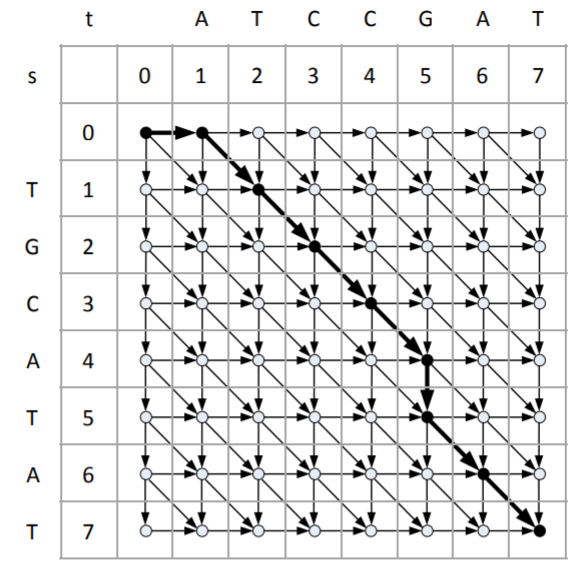
\includegraphics[width=\linewidth]{slike/grafPoravnanja.PNG}
	\centering
	\caption{Mreža poravnanja za nizove \textit{s=TGCATAT}} i \textit{t=ATCCGAT}
	\label{fig:grafPoravnjanja}
\end{figure}


Međutim bitno je istaknuti kako algoritam računanja udaljenosti nije bio prvi efikasni algoritam koji rješava problem poravnanja dva niza. Zbog potreba biologije, biologe je zanimala maksimalna sličnost bioloških sljedova. Needleman i Wunsch prvi su koji su formulirali algoritam za njegovo rješavanje temeljen na dinamičkom programiranju.
 

"Ako želimo s tim algoritmima poravnati genome čovjeka i miša duge nekoliko milijardi baza
trebat će nam minimalno $9\cdot10^{18}$ operacija. Uz radni takt od 1GHz za računanje ovoga
poravnanja trebat će nam preko 200 godina."[Šikić, Domazet-Lošo, Bionformatike, 2013.]
Nažalost, spomenuti algoritmi nisu učinkoviti kada je potrebno usporediti cijele genome, a kamoli više genoma odjednom. Prikladniji pristup rješavanju toga problema su heuristički algoritmi.

"Poravnavanje više sljedova odjednom (engl. multiple sequence alignment; MSA) ima
smisla kada su sljedovi ili neki njihovi dijelovi homologni."[Šikić, Domazet-Lošo, Bioinformatika, 2013.]. Za razliku od uspredbe ulaznog slijeda s bazom podataka, gdje je homologiju potrebno tek odrediti, kod rješavanja poravnanja više sljedova odjednom polazi se od pretpostavke da su sljedovi koje želimo poravnati homologni. Kada su sljedovi homologni cijelom svojom  duljinom i podjednake duljine, radi se o globalnom poravnanju više sljedova odjednom, poput poravnanja genoma više sojeva bakterija. Nasuprot tome, kada su sljedovi homologni samo po dijelovima, mogu se poravnati po sačuvanim dijelovima (engl. \textit{conserved regions}) i tada se radi o lokalnom poravnanju, primjerice poravnanje homolognih proteina između različitih vrsta.
Na slici \ref{fig:msaWiki} prikazan je primjer poravnjanja.

\begin{figure}[htb]
	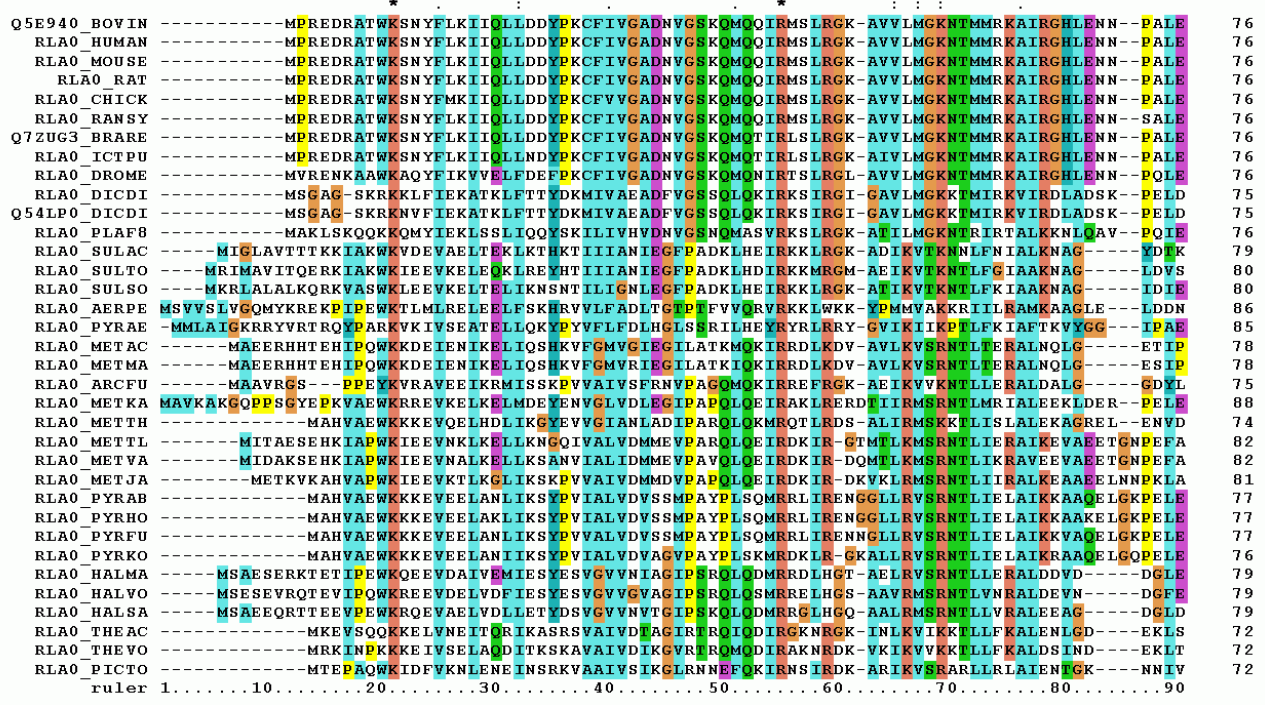
\includegraphics[width=\linewidth]{slike/msaWiki.PNG}
	\centering
	\caption{Poravnanje prvih 90 stupaca proteina L10E iz raznih organizama }
	\label{fig:msaWiki}
\end{figure}

Kod poravnanja tri ili više sljedova odjednom ideja je smjestiti homologna mjesta u promatranim sljedovima u iste stupce. 
\begin{figure}[htb]
	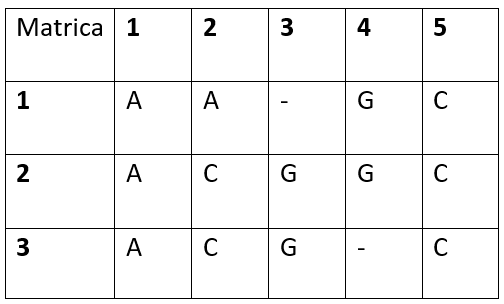
\includegraphics[]{slike/msaPrv.PNG}
	\centering
	\caption{Smještanje homolognih mjesta u iste stupce}
	\label{fig:msaPrv}
\end{figure}
Slika ~\ref{fig:msaPrv} prikazuje jednostavan slučaj poravnanja tri slijeda. Sljedovi su prikazani u matrici, a homologna mjesta smještena su u iste stupce.
Formalna definicija problema jest sljedeća:
neka je zadan skup od \textit{n} sljedova: $S_1, S_2,...,S_n$, abeceda sljedova mogu biti nukleotidi ili aminokiseline. Poravnanje više sljedova odjednom je skup sljedova $S_1',...,S_n'$ za koje vrijedi:
\begin{enumerate}
	\item Duljine poravnatih sljedova su jednake, $|S_1'|=...=|S_n'|$
	\item Uklanjanje praznina "-" iz $S_i'$ dobiva se $S_i$ za \textit{i=1,...,n}	
\end{enumerate}
Moguće je da duljine poravnatih sljedova budu dulje ukoliko su dodavane praznine u početne sljedove.

Heuristički pristupi poravnanju više sljedova odjednom su:
\begin{enumerate}
	\item progresivno poravnanje (engl. \textit{progressive alignment})
	\item metode temeljene na skrivenim Markovljevim modelima (engl. \textit{Hidden Markov Model;} HMM)
	\item iterativne metode
	\item metode temeljene na filogenetskom predznanju
	\item metode temeljene na genetskom algoritmu
\end{enumerate}

Primjer progresivne metode jest alat ClustalW/ClustalX (Thompson et al., 1994; Larkin et al., 2007) te višeprocesorska verzija Clustal Omega(Sievers et al., 2011). Pimjer korištenja iterativne metode jest program MUSCLE (Edgar, 2004.). Primjer korištenja genetskog algoritma za poravnanje više sljedova odjednom izložen je u poglavlju koje opisuje implementaciju ovoga rada.

\renewcommand{\lstlistingname}{Isječak koda}
\lstset{language=C++, tabsize=2, numbers = left, stepnumber=1, showstringspaces=false, basicstyle=\footnotesize}
\chapter{Razvojno okruženje za evolucijsko računanje}
\label{ecf}
ECF (engl. \textit{Evolutionary Computation Framework}) skup je gotovih programa napisanih u programskome jeziku C++ razvijenih na Zavodu za elektroniku, mikroelektroniku, računalne i inteligentne sustave namijenjenih za izradu evolucijskih algoritama.
Neki od ponuđenih algoritama u ECFu su:
\begin{itemize}
	\item genetski algoritam, genetsko programiranje
	\item algoritam roja čestica
	\item algoritam genetsko kaljenje
	\item algoritam kolonije pčela
	\item evolucijska strategija
	\item diferencijska evolucija
\end{itemize}

Za korištenje ECFa prethodno je potrebno preuzeti \textit{boost C++(www.boost.org)}. ECF pruža podršku za Visual Studio i CLion razvojna okruženja. Više detalja oko instalacije moguće je pronaći na \textit{http://ecf.zemris.fer.hr/install.html}.
Za uspješno pokretanje ECFa potrebno je kao argument predati konfiguracijsku datoteku kojom se parametrizira izvođenje. Moguće je parametrizirati genotip, odnosno reprezentaciju jedinke. Trenutna verzija ECFa za genotip nudi \texttt{BitString, FloatingPoint, Binary genotype,  Tree genotype i Permutation genotype}. Uz genotip moguće je odabrati algoritam izvođenja. 

 Primjer korištene konfiguracijske datoteke \texttt{parameters.txt} koju je prilikom pokretanja programa  potrebno predati kao argument dan je na ~\ref{fig:param}.
\begin{figure}[!httb]
	
	\begin{verbatim}
	<ECF>
	  <Algorithm>
	    <SteadyStateTournament>
	      <Entry key="tsize">3</Entry>
	    </SteadyStateTournament>
	  </Algorithm>
	
	  <Genotype>
	    <MsaGenotype>
	      <Entry key="mut.insert">0.33</Entry>
	      <Entry key="mut.delete">0.33</Entry>
	      <Entry key="mut.simple">0.34</Entry>
	    </MsaGenotype>
	  </Genotype>
	
	  <Registry>
	    <Entry key="input">FASTA.txt</Entry>
	  </Registry>
	</ECF>
	\end{verbatim}
	\caption{\texttt{parameters.txt} datoteka}
	\label{fig:param}
\end{figure}
 Konfiguracijska datoteka sastoji se od tri glavne sekcije \texttt{Algorithm, Genotype, Registry}. Jedino je \texttt{Genotype} sekciju nužno definirati u svakoj konfiguracijskoj datoteci, za sve ostale parametre postoje predpostavljene vrijednosti. Sekcija \texttt{Algorithm} služi za odabir željenog algoritma te postavljanje dodatnih parametara poput veličine turnirkse selekcije, odabira elitizma ili maksimalnog broja iteracija. Unutar sekcije \texttt{Genotype} odabire se željena reprezentacija jedinke uz željene parametre specifične za pojedini algoritam. Vrlo često se postavljaju parametri vjerojatnosti pojedinih operatora mutacije. Sekcija \texttt{Registry} sadrži sve parametre nevezane za \texttt{Algorithm} ili \texttt{Genotype}, poput ulazne datoteke, definiranje maksimalnog vremena izvođenja i brojnog drugog.
 
 Primjer evaluacijske funkcije koju je potrebno evaluirati prilikom svakog korištenja razvojnog okruženja ECF nalazi se na ~\ref{fig:eval}. Prikazana evaluacijska funkcija vrednuje bolje rješenje koje ima više jedinica u \texttt{Bitstring} genotipu.
 
 \begin{figure}[!httb]
 	
 	\begin{verbatim}

 	FitnessP OneMaxEvalOp::evaluate(IndividualP individual)
 	{
 	  // evaluation creates a new fitness object (using a smart pointer)
 	  // in our case, we try to maximize the number of ones
 	  FitnessP fitness (new FitnessMax);
 	
 	  // Each individual is a vector of genotypes .
 	  // We'll use BitString, and retrieve it as the first and 
 	  only genotype
 	  BitString::BitString* bitstr = (BitString::BitString*) individual->
 	  getGenotype(0).get(); 
 	
 	  // count the ones; where are they?
 	  // BitString genotype contains a std::vector of bool's named 'bits'
 	  uint ones = 0;
 	  for(uint i = 0; i<bitstr->bits.size(); i++){
 	    if(bitstr->bits[i] == true)
 	      ones++ ;
 	  }
 	  fitness->setValue(ones);
 	
 	  // return the new fitness
 	  return fitness;
 	}
 	\end{verbatim}
 	\caption{Primjer evaluacijske funkcije iz  \cite{ecfManual}}
 	\label{fig:eval}
 \end{figure}
 


\renewcommand{\lstlistingname}{Isječak koda}
\lstset{language=C++, tabsize=2, numbers = left, stepnumber=1, showstringspaces=false, basicstyle=\footnotesize}
\chapter{Implementacija genetskog algoritma za odabrani problem} \label{implementacija}
Koristeći razvojno okruženje za evolucijsko računanje Evolutionary Computation Framework - ECF riješen je problem poravnanja tri ili više DNK/RNK slijeda odjednom. Za rješavanje poravnanja aminokiselina potrebno je nadograditi algoritam na način objašnjen u nastavku.

\section{Populacija}
Kako bi unutar ECFa rješili neki optimizacijski problem potrebno je unutar konfiguracijske datoteke zadati i odabrati genotip jedinke. S obzirom da ECFova trenutna implementacija sadrži razrede \texttt{BitString, FloatingPoint, Binary genotype,  Tree genotype i Permutation genotype} te nijedan genotip nije prikladan za reprezentaciju jedinke osmišljen je novi genotip. Novi genotip \texttt{MsaGenotype} nasljeđuje osnovni razred \texttt{Genotype} te sadrži atribut \texttt{vector<string> alignment} čime je reprezentirana jedinka.
Virtualna metoda koju je potrebno naslijediti kako bi se napravio novi genotip jest metoda \texttt{initialize(StateP state)}. U toj metodi implementirano je generiranje inicijalne populacije.
Prvim pokretanjem metode \texttt{initialize} \texttt{FastaParser.cpp} pročita datoteku zadanu kao parametar u konfiguracijskoj datoteci \texttt{<Entry key="input">FASTA.txt</Entry>} pod sekcijom \texttt{Registry} zapisanu u FASTA formatu podataka te odredeđuje najdulji niz. Nakon toga početna duljina svakog slijeda generira se na način da se u slijed umeću praznine na slučajno odabranom mjestu dok duljina slijeda ne postane 10\% dulja od duljine najduljeg niza. Sljedeći primjer daje mogući izgled FASTA.txt datoteke te generirane jedinke.


\begin{verbbox}
	>first
	ATTGCCGACT
	>second
	AC
	>third
	GACCCTAG
\end{verbbox}
\begin{figure}[ht]
\centering
\theverbbox
\caption{\textit{FASTA.txt} datoteka}
\end{figure}

\begin{verbbox}
	ATTGC-CGACT
	--A----C---
	G--A-CCCTAG
\end{verbbox}
\begin{figure}[ht]
	\centering
	\theverbbox
	\caption{Generirana jedinka}
\end{figure}
Opisani način generiranja inicijalne populacije odgovara autorima Horng et al. (2005), Shyu et al. (2004) i Wang \& Lefkowitz (2005), dok 
Hernandez et al. (2004) već prilikom inicijalnog generiranja jedinki radi djelomično poravnanje.

\section{Reprodukcija}

Autori  (Hernandez et al., 2004; Horng et al., 2005; Shyu et al.,2006; Wang \& Lefkowitz, 2005) koriste jednstavnu turnirsku selekciju (engl. \textit{roulette wheel parent seelction}). Autori (Horng et al., 2006; Wang \&Lefkowitz, 2005) također koriste neki oblik elitizma kako bi sačuvali najbolju jedinku. Čiji je pseudokod dan u nastavku

\begin{figure}[h]

\begin{verbatim}
single generation {
   select individuals to form the new generation /
   		(fitness proportional selection operator);
   create new generation (make copies);
   noCrx = (deme size) * <crxRate_> / 2;
   repeat(<noCrx> times) {
      randomly select two parents;
      perform crossover, _replace_ parents with their children;
   }
   perform mutation on new generation;
}
\end{verbatim}
	\caption{Pseudokod genetskog algoritma s jednostavnom selekcijom(\texttt{roulette wheel}) u  razvojnom okruženju ECF}
\end{figure}

 U implementaciji rješenja u razvojnom okruženju ECF korištena je 3-turnirsku eliminacijsku selekciju čiji je pseudokod dan u nastavku:
 
 \begin{figure}[h]

 \begin{verbatim}
 	single generation {
 	   repeat(deme size times) {
 	      randomly add <nTournament_> individuals to the tournament;
  	      select the worst one in the tournament;
 	      randomly select two parents from /
 	      		remaining ones in the tournament;
 	      replace the worst with crossover child;
 	      perform mutation on child;
 	   }
 	}
 \end{verbatim}
  	\caption{Pseudokod eliminacijskog genetskog
  		algoritma s jednostavnom troturnirskom selekcijom(\texttt{steady state tournament}) algoritma u razvojnom okruženju ECF}
\end{figure}
 
 Oba navedena algoritma implementirana su u ECFu, a odabir algoritma naveden je \texttt{Algorithm} sekciji na sljedeći način prikazan na ~\ref{algSekcija}
 \begin{figure}
 	
 \begin{verbatim}
 <SteadyStateTournament>
 	<Entry key="tsize">3</Entry>               
 </SteadyStateTournament>
 \end{verbatim}
\caption{\texttt{Algorithm} sekcija u ECFu za odabir željenog algoritma}
\label{algSekcija}
\end{figure}
 
 \section{Križanje}
 Kako bi se u ECFu implementirao operator križanja (engl. \textit{crossover}) potrebno je naslijediti klasu \texttt{CrossoverOp} te implementirati zadanu metodu \texttt{mate(GenotypeP gen1, GenotypeP gen2, GenotypeP child)}. Implementacija križanja s jednom točkom prekida dana je u \texttt{MsaGenotypeCrsOnePoint}. Budući da dvije jedinke koje se križaju ne moraju imati sljedove jednake duljine, slučajno se odabire točka prekida na jedinci s kraćim slijedovima. Točka prekida slučajno se generira sve dok nije zadovoljen uvjet da jedinka sadrži nizove veće ili jednake duljine niza od najveće pronađene duljine niza prilikom čitanja datoteke FASTA.txt. Time se sprječava konvergencija genetskog algoritma prema rješenju koje biološki nema smisla kod poravnanja sljedova, iako ga evaluacijska funkcija može vrednovati kao bolje rješenje. Primjer križanja dan je na ~\ref{fig:krizanje}. Oznaka "|" predstavlja odabranu točku prekida. Dijete u ovome slučaju sadrži genetskog materijal prvog roditelja do točke prekida, a od točke prekida sadrži genetski materijal drugog roditelja. Nakon toga uklanjaju se stupci koji sadrže isključivo praznine.
 \begin{figure}
 \begin{verbatim}
Roditelj 1  Roditelj 2     Dijete
 	AT|CG-A     GG|GC-TA     AT|GC-TA
 	CG|T--G	 +  TA|-GACG  =  CG|-GACG
 	GA|TC--	     CG|--GGA     GA|--GGA
 \end{verbatim}
 \caption{Primjer križanja}
 \label{fig:krizanje}
\end{figure}
 
 Kod funkcije \texttt{mate} dan je u nastavku:
 
 
 \begin{lstlisting}[caption=Funkcija \texttt{mate}]
 	bool MsaGenotypeCrsOnePoint::mate(GenotypeP gen1, GenotypeP gen2, GenotypeP child)
 	{
 	   // dohvat roditelja i djeteta
 	   MsaGenotype *p1 = (MsaGenotype *) (gen1.get());
 	   MsaGenotype *p2 = (MsaGenotype *) (gen2.get());
 	   MsaGenotype *ch = (MsaGenotype *) (child.get());
 		
     // generiraj tocku prekida na kracem slijedu
 	   int cross_point = state_->getRandomizer()->
 	     getRandomInteger(std::min(p1->alignment[0].size(), 
 	      p2->alignment[0].size()));
 	
 	   // slucajno odaberi raspored prepisivanja
 	   // genetskog materijala roditelja
 	   switch (state_->getRandomizer()->getRandomInteger(0, 1)) {
 	   case 0: // prvo zapisi prvog roditelja
 	
 	   for(int i = 0; i < p1->alignment.size(); i++)
 	   {
 	     ch->alignment[i] = p1->alignment[i].substr(0, cross_point) 
 	       + p2->alignment[i].substr(cross_point);
 	     std::cout << p1->alignment[i].substr(0, cross_point) +
 	      p2->alignment[i].substr(cross_point) << "\n";
 	   }
 	   break;
 	   case 1: // prvo zapisi drugog roditelja
 	   for (int i = 0; i < p1->alignment.size(); i++)
 	   {
 	     ch->alignment[i] = p2->alignment[i].substr(0, cross_point) 
 	       + p1->alignment[i].substr(cross_point);
 	   }
 	   }
 	   // ukloni stupce sa iskljucivo prazninama
 	    	
 	}
 \end{lstlisting}

 
 \section{Mutacija}
 Operatori mutacije u ECFu ostvaruju se nasljeđivanjem razreda \texttt{MutationOp}. U implementaciji su ponuđene tri različita operatora mutacije: \texttt{MsaGenotypeMut, MsaGenotypeMutDeleteGap, MsaGenotypeMutInsertGap}. Svi autori se slažu kako su ključne mutacije brisanje i umetanje praznina, međutim implementiraju to na različite načine.
 
 \texttt{MsaGenotypeMut} po uzoru na Shyu et al. (2004) slučajno odabire dva stupca te u svakome sljedu zamjenjuje sadržaj tih stupaca.
 \begin{lstlisting}[caption=Jednostavna mutacija izmjene stupaca]
 bool MsaGenotypeMut::mutate(GenotypeP gene) {
  // dohvati jedinku
 	MsaGenotype* msa_alignment = (MsaGenotype*) (gene.get());
 
  // odaberi prvu poziciju
 	int first_position = state_->getRandomizer()->
 	getRandomInteger(msa_alignment->
 	getAlignment().size());
 	// odaberi drugu poziciju
 	int second_position = state_->getRandomizer()->
 	getRandomInteger(msa_alignment->
 	getAlignment().size());
  		
  	std::vector<std::string> &alignment = msa_alignment->
  	getAlignment();
 // zamijeni stupce na pozicijama jedan i dva 
 	for (int i = 0; i < alignment.size(); i++)
 	{
 		if (state_->getRandomizer()->getRandomInteger(2))
 		  std::swap(alignment[i][first_position],
 		   alignment[i][second_position]);
 	}
 
 	return true;
}
 \end{lstlisting}
 
 \begin{figure} [httb]
	\begin{verbatim}
		ACG-GTA  Mutacija  ACG-GTA
		AGCGGTA ---------> ACGGGTA
		-CAG--A            -CAG--A
	\end{verbatim}
	\caption{Primjer djelovanja operatora jednostavne mutacije}
	\label{fig:jednostavnaMutacija}
 \end{figure}

Primjer ~\ref{fig:jednostavnaMutacija} ilustrira jednostavnu mutaciju. U prvome retku slučajno su odabrane dvije jednake pozicije te se mutacija nije dogodila. U drugome retku odabrane su pozicije 1 i 2, dok su utrećem retku odabrane pozicije 0 i 4. U prvome retku i trećem retku efekt je kao da se nije ni dogodila mutacija, dok mutacija u drugome retku osigurava bolje poravnanje.

 Operator mutacije \texttt{MsaGenotypeMutInsertGap} za svaki slijed odabire slučajnu poziciju te umeće prazninu.
 \begin{lstlisting} [caption= Mutacija umetanja praznina]
 	bool MsaGenotypeMutInsertGap::mutate(GenotypeP gene)
 	{
 	   // dohvati jedinku
 	   MsaGenotype* msa_alignment = (MsaGenotype*) (gene.get());
 	   std::vector<std::string> &alignment = msa_alignment->
 	   getAlignment();
 	   // za svaki redak slucajno odaberi poziciju 
 	   // na odabranu poziciju umenti prazninu
 	   for (int i = 0; i < alignment.size(); i++)
 	   {
 	     int pos = state_->getRandomizer()->
 	     getRandomInteger(alignment[i].size() + 1);
 	     alignment[i].insert(pos, "-");
 	   }
 	   return true;
 	}

 \end{lstlisting}
 
  \begin{figure} [httb]
 	\begin{verbatim}
 	ACG-GTA  Mutacija  AC-G-GTA
 	AGCGGTA ---------> AGCGG-TA
 	-CAG--A            -CAG---A
 	\end{verbatim}
 	\caption{Primjer djelovanja operatora umetanja praznina}
 	\label{fig:umetanje}
 \end{figure}
 Primjer ~\ref{fig:umetanje} prikazuje djelovanje operatora umetanja praznina, koje za ovaj slučaj povećava vrijednost evaluacijske funkcije. U prvome retku praznina se umeće na poziciju 2, u drugome retku na poziciju 4, dok u trećem retku se umeće na poziciju 5.
  Operator \texttt{MsaGenotypeMutDeleteGap} prvo provjerava postoji li u svakome slijedu praznina. Ukoliko je taj uvjet zadovoljen, za svaki slijed se određuju indeksi praznina, te nakon toga slučajno odabire jedan od pronađenih indeksa na kojem će se izbrisati praznina.
  \begin{lstlisting} [caption=Mutacija brisanja praznina]
bool MsaGenotypeMutDeleteGap::mutate(GenotypeP gene)
{
  // dohvati jedinku
   MsaGenotype* msa_alignment = (MsaGenotype*) (gene.get());
   std::vector<std::string> &alignment = msa_alignment->
   getAlignment();
   // prvjeri postoji li praznina u svakom retku
   bool no_gap = false;
   for (int i = 0; i < alignment.size(); i++)
   {
      if (alignment[i].find('-') == std::string::npos)
      {
         no_gap = true;
         break;
      }
   }
   // ako je pronadjen redak bez praznine
   // ne obavljaj mutaciju
   if (no_gap) return true;
   for (int i = 0; i < alignment.size(); i++)
   {
     // pronadji indekse praznina
      std::vector<int> indexes;
      int br = 0;
      for(auto& c : alignment[i])
      {
         if(c == '-')
         {
           indexes.push_back(br);
         }
         br++;
      }
      int pos = state_->getRandomizer()->
      getRandomInteger(indexes.size());
      // obrisi prazninu na slucajnoj poziciji
      alignment[i].erase(alignment[i].begin() + indexes[pos]);
	    indexes.clear();
   }
   return true;
}
  \end{lstlisting}
  
  
  \begin{figure} [httb]
  	\begin{verbatim}
  	ACGG-GTA  Mutacija   ACGGGTA
  	AG-CGGTA --------->  AGCGGTA
  	-CAG--A-             -CAG--A
  	\end{verbatim}
  	\caption{Primjer djelovanja operatora brisanja praznina}
  	\label{fig:brisanje1}
  \end{figure}
 Slika ~\ref{fig:brisanje1} prikazuje primjer djelovanja operatora brisanja praznina, zadovoljen je uvjet da svaki redak sadrži prazninu. U prvome retku briše se jedina moguća praznina, u drugome retku briše se praznina na poziciji 2, dok se u trećem retku briše ravnina na poziciji 7.
  
  \begin{figure} [httb]
  	\begin{verbatim}
  	ACG-GTA  Mutacija  ACG-GTA
  	AGCGGTA ---------> AGCGGTA
  	-CAG--A            -CAG--A
  	\end{verbatim}
  	\caption{Primjer djelovanja operatora brisanja praznina bez promjene}
  	\label{fig:brisanje2}
  \end{figure}

U primjeru na slici ~\ref{fig:brisanje2} nije zadovoljen uvjet da se u svakome retku nalazi praznina te stoga nema promjene nad jedinkom. Kada se nebi ispitivao uvjet da se u svakome retku nalazi praznina dobili bismo jedinku s retcima različitih duljina koju ne možemo vrednovati evaluacijskom funkcijom, niti bi takvo rješenje imalo smisla.
  
  
  \section{Evaluacijska funkcija}
  
  Evaluacijska funkcija određuje koliko je pojedino rješenje, to jest jedinka kvalitetno. Implementacija funkcije dobrote predstavlja najveći izazov prilikom rješavanja poravnanja više sljedova odjednom genetskim algoritmom. U literaturi sve funkcije dobrote svode se na metodu sume parova.
  Navedenu metodu moguće je ostvariti na dva načina:
  \begin{enumerate}
  	\item Uspoređivanjem svakog para elemenata u određenom stupcu. Za preklapajuće dušične baze ukupnoj sumi se pridodaje jedan. Za neodgovarajuće baze sumi se dodaje -1. Ukoliko je bilo koji od uspoređivanih parova jednak praznini "-" sumi se dodaje -2. Ova jednostavna implementacija proširiva je korištenjem BLOSUM i PAM matrica za podršku poravnanja aminokiselina, a ne samo DNA i RNA sljedova.
  	\item Određivanjem elementa s najvećim brojem ponavljanja za svaki stupac te uspoređivanjem ostalih elemenata stupca s tim elementom.
  \end{enumerate}

 U implementaciji rješenja korištena je jednostavna usporedba navedena pod točkom 1. bez podrške za aminokiseline. Slika \ref{fig:tablicaEvaluacije} prikazuje primjer poravnanja reprezentiran matricom kako bi se opisao postupak izračuna funkcije dobrote. Primjer izračuna za \ref{fig:tablicaEvaluacije} dan je u nastavku.

\begin{figure}[h]
	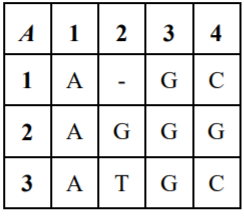
\includegraphics[]{slike/tablicaEvaluacije.PNG}
	\centering
	\caption{Primjer poravnanja za objašnjenje izračuna evaluacijske funkcije}
	\label{fig:tablicaEvaluacije}
\end{figure}


\[SP(A_1) = s(A_{1,1}, A_{2,1}) + s(A_{1,1}, A_{3,1}) + s(A_{2,1},A_{3,1}) = 1 + 1 + 1 = 3\]
\[SP(A_2) = s(A_{1,2}, A_{2,2}) + s(A_{1,2}, A_{3,2}) + s(A_{2,2},A_{3,2}) = -5\]
\[SP(A_3) = s(A_{1,3}, A_{2,3}) + s(A_{1,3}, A_{3,3}) + s(A_{2,3},A_{3,3}) = 3\]
\[SP(A_4) = s(A_{1,4}, A_{2,4}) + s(A_{1,4}, A_{3,4}) + s(A_{2,4},A_{3,4}) = -1\]
\[SP(A) = SP(A_1) + SP(A_2) + SP(A_3) + SP(A_4) = 0\]

Kako bi implementirali funkciju dobrote u ECFu potrebno je naslijediti klasu \texttt{EvaluateOp} i implementirati metodu \texttt{FitnessP evaluate(IndividualP individual)}
 Implementacija metode dana je u nastavku:
 \begin{lstlisting} [caption=Implementacija evaluacijske funkcije]
 	FitnessP MsaEvalOp::evaluate(IndividualP individual)
 	{ 
 		FitnessP fitness(new FitnessMax);
 		MsaGenotype::MsaGenotype* msagen = (MsaGenotype::MsaGenotype*) individual->
 		  getGenotype().get();
 		std::vector<std::string> alignment = msagen->getAlignment();
 		int sum = 0;
 		int num_of_columns = alignment[0].size();
 		int num_of_sequences = alignment.size();
 		for (int column = 0; column < num_of_columns; column++)
 		{
 			for (int i = 0; i < alignment.size() - 1; i++)
 			{
 				std::string current_sequence = alignment[i];
 				if (current_sequence[column] == '-')
 				{
 					sum += (num_of_sequences - i - 1) * gaps;
 					continue;
 				}
 				for (int j = i+1; j < alignment.size(); j++)
 				{
 					if (current_sequence[column] == alignment[j][column])
 						sum += match;
 					else if (alignment[j][column] == '-')
 						sum += gaps;
 					else
 						sum += mis_match;
 				}
 		}
 		fitness->setValue(sum);
 	}
 \end{lstlisting}
  
  Kako bi se postignula što kvalitetnija implementacija koja bi se čim više pibližila alatim poput Clustal Omega potrebno je implementirati funkciju dobrote koristeći biološka saznanja.\newline
  
  
 
  

\chapter{Usporedba ostvarenih rezultata} \label{rezultati}
Na sljedećoj slici ~\ref{fig:svaTruOperatora} vidljiv je rezultat pokretanja implementacije genetskog algoritma za prethodno navedenu FASTA.txt datoteku. Operatori mutacije biraju se jednakim vjerojatnostima svakog puta, to se moglo postići i ne navođenjem nijednog operatora mutacije u konfiguracijskoj datoteci.



 \begin{figure} [httb]
	\begin{verbatim}
	Best of run:
	<HallOfFame size="1">
	  <Individual size="1" gen="0">
	    <FitnessMax value="-48"/>
	    <MsaGenotype size="3">
	ATTGCCG-ACT-
	--------AC--
	-GACCCT-AG--
    </MsaGenotype>
  </Individual>
</HallOfFame>
	\end{verbatim}
	\caption{Poravnanje FASTA.txt koristeći sva tri operatora mutacije}
	\label{fig:svaTruOperatora}
 \end{figure}

Sljedeća slika prikazuje poravnanje iste ulazne datoteke koristeći alat Clustal Omega

\begin{figure}[h]
	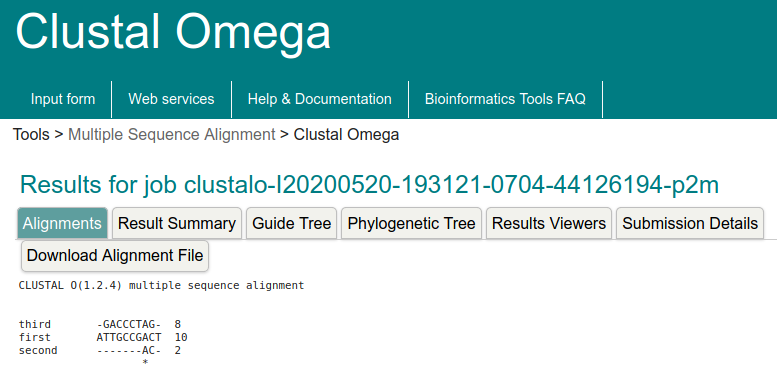
\includegraphics[]{slike/clustalMali.PNG}
	\centering
	\caption{Poravnanje FASTA.txt pomoću Clustal Omege}
	\label{fig:clustalMali}
\end{figure}

Vidljivo je kako implementacija genetskog algoritma ne pronalazi globalni maksimum, već ostane na pronađenome lokalnome maksimumu.

Prethodni rezultati dobiveni su genetskim algoritmom koristeći operatore mutacije s jednakom vjerojatnošću.

Sljedeće slike prikazuju rezultate izvođenja kada se koristi samo operator mutacije brisanja praznina.



\begin{figure} [httb]
\begin{verbatim}
Best of run:
<HallOfFame size="1">
  <Individual size="1" gen="1">
    <FitnessMax value="-37"/>
      <MsaGenotype size="3">
ATTGCCGACT
--AC------
GGACCCT-AG
</MsaGenotype>
  </Individual>
</HallOfFame>
\end{verbatim}
\caption{Poravnanje FASTA.txt koristeći samo operator mutacije brisanja praznina}
\label{fig:samoDelete}
\end{figure}

Iz slike ~\ref{fig:samoDelete} vidljivo je kako u malenome primjeru korištenjem samo operatora mutacije, postiže se rezultat s većom vrijednošću funkcije dobrote. Naravno, u primjerima gdje nije velika razlika u početnim duljinama sljedova, operator mutacije brisanja neće znatno doprinijeti rješenju. Shodno tome bolje rješenje na velikim primjerima postići će se korištenjem svih triju operatora mutacije.

Testiranje korištenjem samo operatora mutacije umetanja praznina ili samo operatora zamjene dva stupca rezultiraju na jednaki način. Jedinke dobivene operatorima mutacije imaju manje vrijednosti evaluacijske funkcije u usporedbi s inicijalno generiranom populacijom. Zbog toga što umetanje praznina na bilo koje mjesto samo umanjuje vrijednost funkcije dobrote, iako uz kombinaciju s drugim operatorima ta jedinka s umetnutim prazninama može pridonjeti pronalasku novog najboljeg pronađenog rješenja. 
Ostale kombinacije svih triju operatora mutacije, gdje je vjerojatnost odabira pojedinog dvostruko veća od sume vjerojatnosti preostala dva operatora rezultiraju na relativno jednaki način, te ne pridonose značajno u pronalasku boljeg rješenja.

Slika ~\ref{fig:gamsaVeliki} prikazuje poravnanje DNA MYH16 sljedova genetskim algoritmom.


\begin{figure}[]
	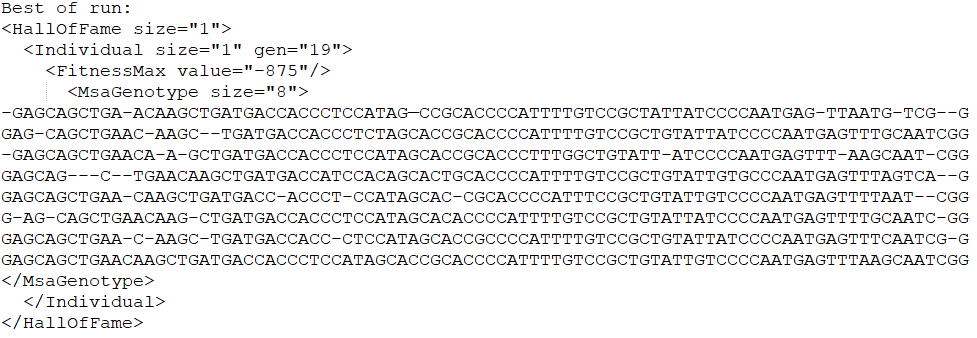
\includegraphics[]{slike/gamsaVeliki2.PNG}
	\centering
	\caption{Poravnanje DNA MYH16 genetskim algoritmom}
	\label{fig:gamsaVeliki}
\end{figure}

Slika ~\ref{fig:clustalVeliki} prikazuje poravnanje DNA MYH16 s Clustal Omegom.  

\begin{figure}[]
	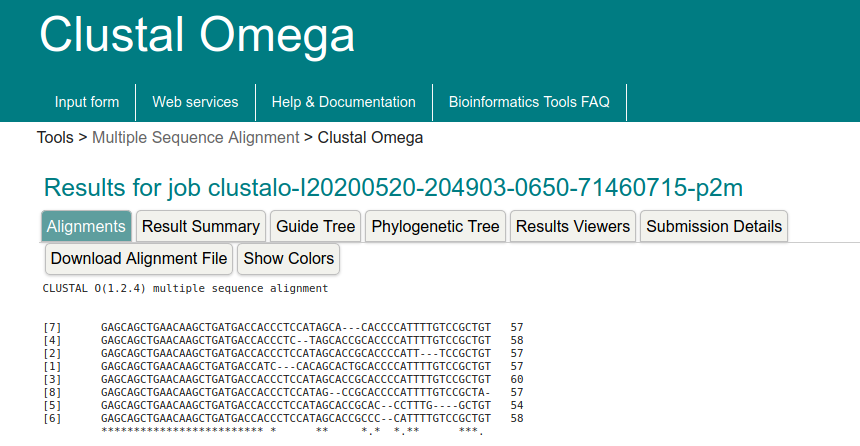
\includegraphics[]{slike/clustalVeliki.PNG}
	\centering
	\caption{Poravnanje DNA MYH16 koristeći Clustal Omega}
	\label{fig:clustalVeliki}
\end{figure}

Usporedbom ~\ref{fig:clustalVeliki} s ~\ref{fig:gamsaVeliki} vidljivo je kako je implementacija Clustal Omege tim više bolja za veće primjere koje je ptrebno rješavati u praksi. 
Genetski algoritam mogao bi se unaprijediti korištenjem još većeg broja operatora mutacije i dodatnih operatora križanja te ono najbitnije korištenjem naprednije funkcije dobrote koja bi koristila biološko predznanje.

\chapter{Zaključak} \label{zakljucak}
U ovom radu dan je kratak uvod u potrebu razvijanja evolucijskog računarstva te time i genetskog algoritma. Predstavljeni su optimizacijski problemi iz područja bioinformatike te je predloženo rješenje genetskim algoritmom.

Opisan je i implementiran problem poravnanja više sljedova odjednom genetskim algoritmom koristeći razvojno okruženje za evolucijsko računanje ECF razvijeno na Fakultetu elektrotehnike i računarstva u Zagrebu.

Iako genetski algoritam postiže dobre rezultate za poravnanje manjeg broja i manje duljine DNA lanaca, razlika između poravnanja uz pomoć alata Clustal Omega koji se temelji na progresivnoj metodi poravnanja postaje veća s većim primjerima .~\nocite{*}


\bibliography{literatura}
\bibliographystyle{fer}

\begin{sazetak}
U ovom radu dan je uvod u evolucijsko računarstvo i genetski algoritam. Opisani su optimizacijski problemi iz bioinformatike. Koristeći Evolutionary Computation Framework genetskim algoritmom pristupilo se problemu poravnanja više sljedova odjednom. Pokazani su nedostaci primjene genetskog algoritma na danome problemu te je ispitana ovisnost o vjerojatnostima operatora mutacije.

\kljucnerijeci{genetski algoritam, optimizacijski problemi, bioinformatika, poravnanje više sljedova odjednom, Evolutionary Computation Framework}
\end{sazetak}


\engtitle{Applications of evolutionary algorithms in bioinformatics}
\begin{abstract}
In this paper an intro to evolutionary computing and genetic algorithm is given. Optimization problems from bionformatics are described. The problem of multiple sequence alignment is solved with genetic algorithm in Evolutionary Computation Framework. Flaws of genetic algorithm are stated on the given problem and the relationship between the probabilities of mutation operators and the quality of solution is estimated.

\keywords{genetic algorithm, optimization problems, bioinformatics, multiple sequence alignment, Evolutionary Computation Framework}
\end{abstract}

\end{document}
